%!TEX root = ../../main.tex
\chapter{性能評価・考察}
本研究の評価として,システムの操作性と推薦機構の評価実験を行った.

\section{実験環境}
// TODO:

\section{システムの操作性の比較実験}
// TODO:

\subsection{実験内容}
\ref{img:experiment_question}に示す.

\begin{figure}[t]
	\begin{center}
		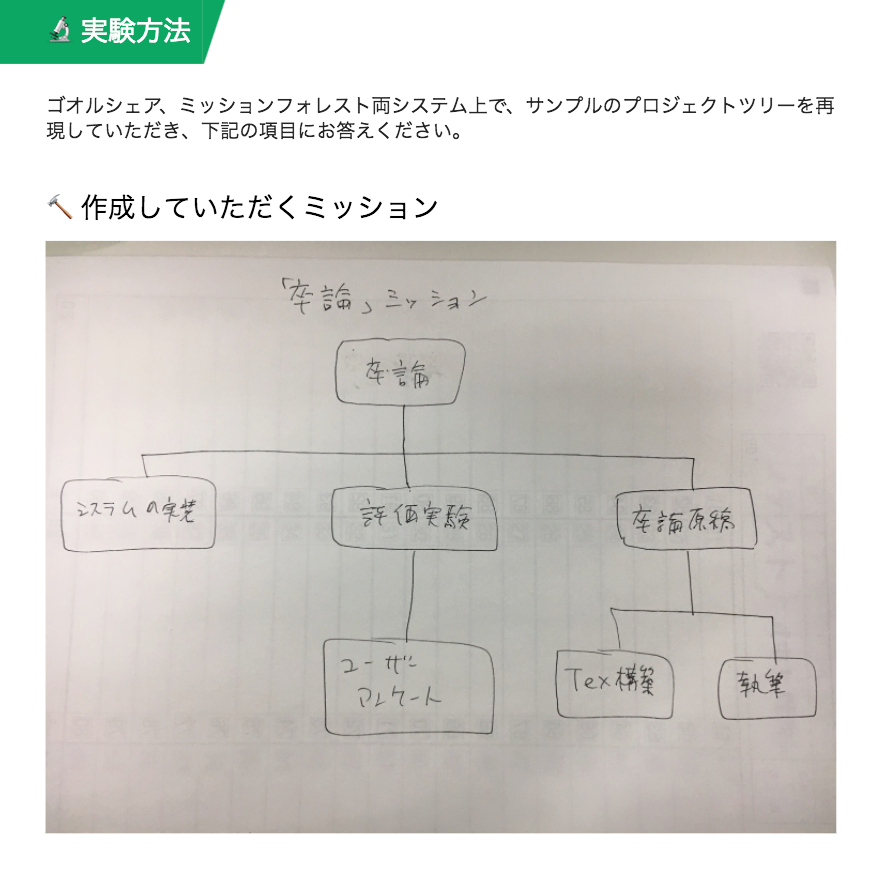
\includegraphics[width=0.9\linewidth]{assets/img/experiment_question.png}
		\caption{評価実験項目}
		\label{img:experiment_question}
	\end{center}
\end{figure}

\subsection{実験結果と考察}

\ref{img:experiment_goalshare}に示す.

\begin{figure}[t]
	\begin{center}
		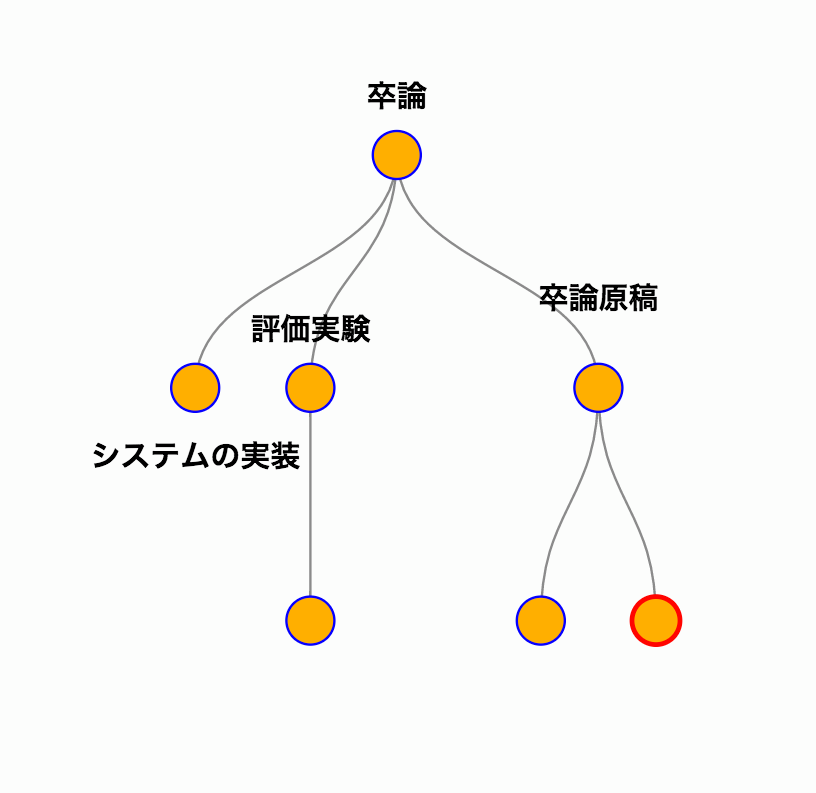
\includegraphics[width=0.9\linewidth]{assets/img/experiment_goalshare.png}
		\caption{ゴオルシェア実験結果}
		\label{img:experiment_goalshare}
	\end{center}
\end{figure}

\ref{img:experiment_missionforest}に示す.

\begin{figure}[t]
	\begin{center}
		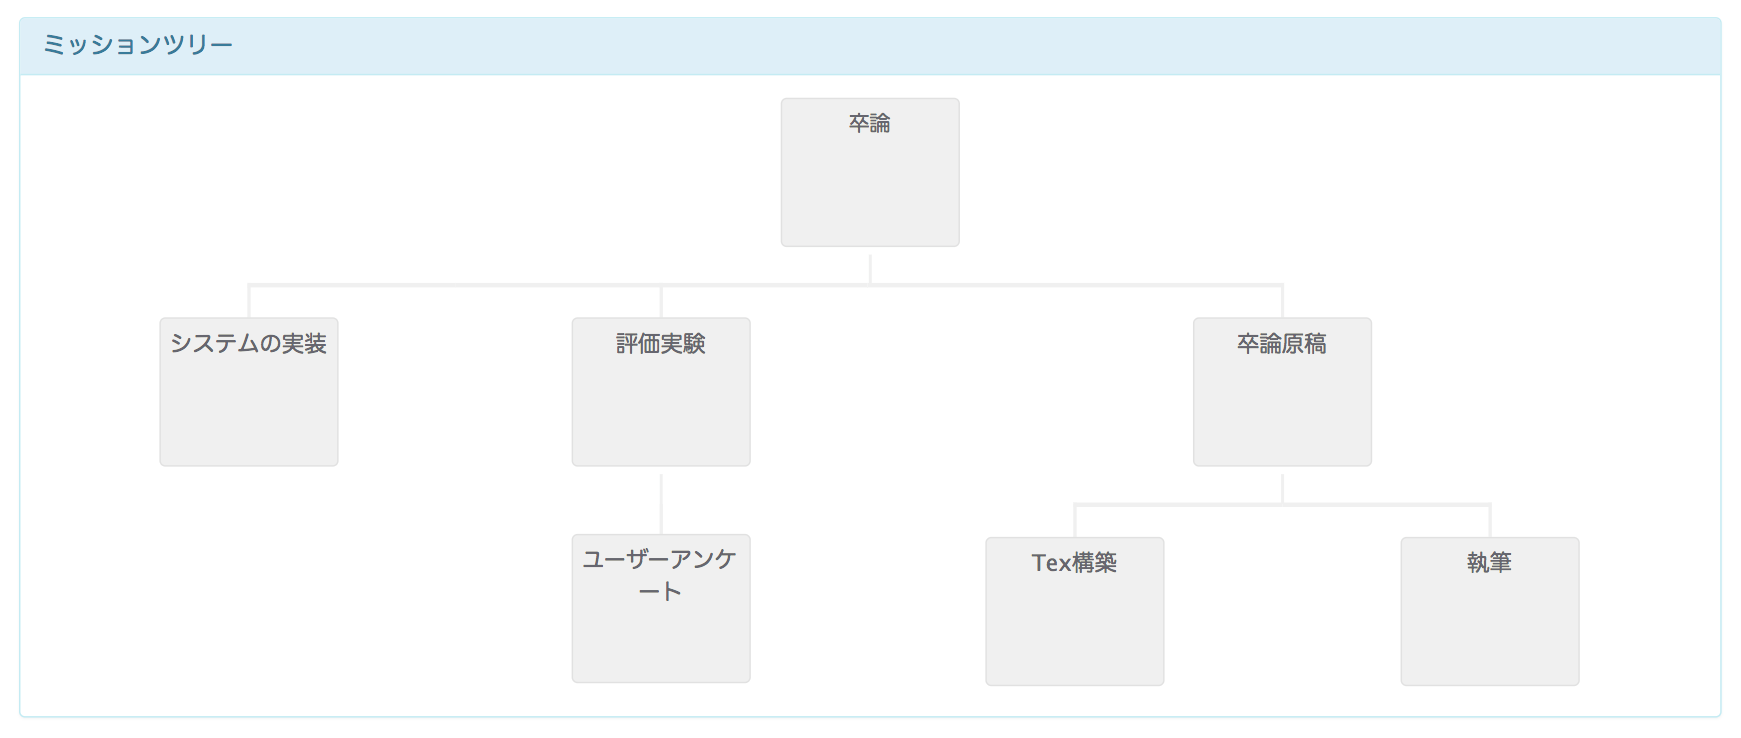
\includegraphics[width=0.9\linewidth]{assets/img/experiment_missionforest.png}
		\caption{ミッションフォレスト実験結果}
		\label{img:experiment_missionforest}
	\end{center}
\end{figure}

\section{推薦機構の精度}
// TODO:

\subsection{実験内容}
// TODO:

\subsection{実験結果と考察}
// TODO:
